\def\putbox#1#2#3#4{\makebox[0in][l]{\makebox[#1][l]{}\raisebox{\baselineskip}[0in][0in]{\raisebox{#2}[0in][0in]{\scalebox{#3}{#4}}}}}
\def\rightbox#1{\makebox[0in][r]{#1}}
\def\centbox#1{\makebox[0in]{#1}}
\def\topbox#1{\raisebox{-0.60\baselineskip}[0in][0in]{#1}}
\def\midbox#1{\raisebox{-0.20\baselineskip}[0in][0in]{#1}}
   \scalebox{1}{
   \normalsize
   \parbox{5.90104in}{
   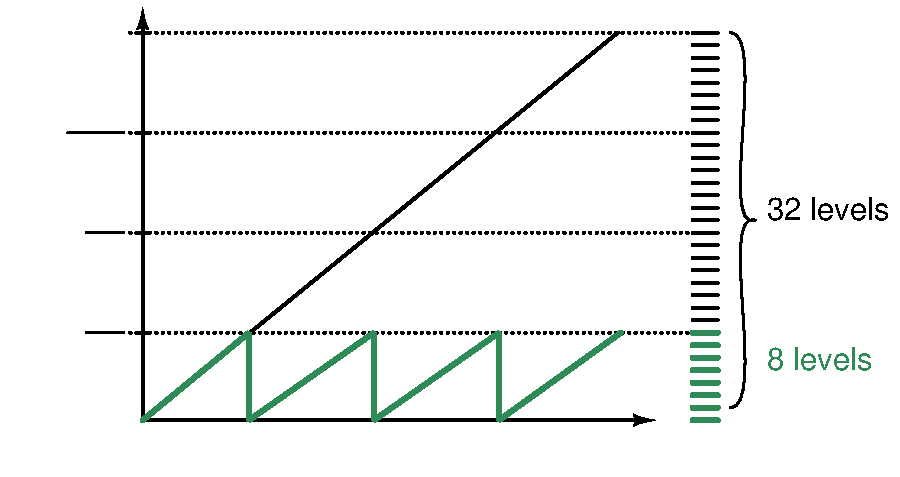
\includegraphics[scale=1]{Chapter3/Figs/folding_signal_principle}\\
   % translate x=364 y=254 scale 0.38
   \putbox{1.70in}{0.09in}{1.20}{Input Voltage [V]}%
   \putbox{0.20in}{0.67in}{1.20}{\rotatebox{-270}{Voltage Processed [V]}}%
   \putbox{0.54in}{1.71in}{0.84}{\(V_{REF}\)}%
   \putbox{0.41in}{2.38in}{0.84}{3}%
   \putbox{0.66in}{1.50in}{0.84}{2}%
   \putbox{0.54in}{1.05in}{0.84}{\(V_{REF}\)}%
   \putbox{0.54in}{2.38in}{0.84}{\(V_{REF}\)}%
   \putbox{0.54in}{2.96in}{0.84}{\(V_{REF}\)}%
   \putbox{0.66in}{0.84in}{0.84}{4}%
   \putbox{0.58in}{2.17in}{0.84}{4}%
   } % close 'parbox'
   } % close 'scalebox'
   \vspace{-\baselineskip} % this is not necessary, but looks better
